\section{Problem Analysis}
\label{sec:problem-analysis}
This section gives an analysis of the problem as defined in the
previous section \ref{sec:problem-definition}. More specifically, this
section describes the problems that are expected and to be solved
during the implementation process of the product. The first part of
this section describes the process of incorporating REPL generation
within the larger context of Spoofax. The second part analyzes the
part of the problem concerned with literate programming, but this part
will be analyzed in less detail than generating REPLs as it is unsure
whether this will be present in the final product.

\subsection{Incorporating REPL generation within Spoofax}
\label{ssec:incorp-repl-gener}
To generate solidly working REPLs for any language defined in Spoofax,
some Spoofax concepts have to be carefully considered. Since every
language can have many different language constructs, generating REPLs
should not be constrained to language specific constructs like
classes, but should rather be done generically. Therefore the
implementation and particularly the interaction with the user needs to
be thought of carefully.

This section lists the problems that are expected when trying to
implement generating REPLs generically. For each problem, their
solution approaches that should be explored during the implementation
process are given, as well as the parts of Spoofax that are relevant
for that problem.

\subsubsection{Detecting unfinished expressions for multiline editing}
\label{sec:detect-unfin-expr}

\subsubsection{Language specific additional commands}
\label{sec:lang-spec-addit}
Another problem is when some additional command can be useful for a
REPL of a particular language, but would not make any sense within the
context of other languages. For example, some languages such as Java
have the notion of a ``module'' or ``package'', which declares a
separate namespace for the definitions in it. An additional command to
list all of the currently loaded modules is useful, but would not make
any sense in languages that have no concept of a module.

This problem could be solved by the language designer by extending his
or her language with reflective capabilities. However in that case it
would not be an additional command, but just an expression like any
other expression in that language. Moreover, the language designer
might not want to extend the language with reflective capabilities
outside of the context of a REPL, for example when the language is a
DSL. It is clear therefore that a different approach should be
considered.

\begin{figure}[htbp]
  \centering
  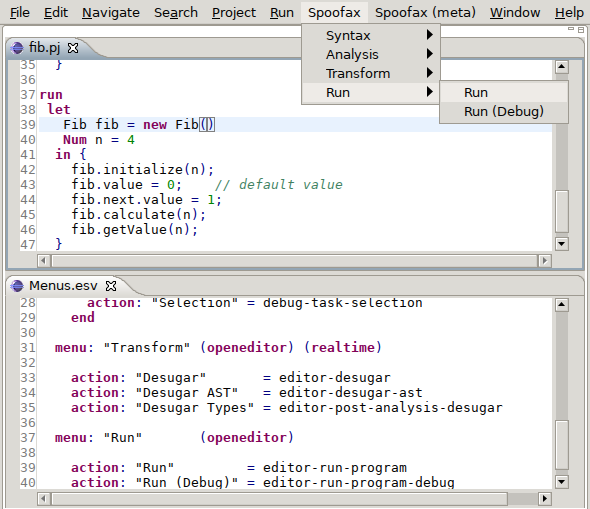
\includegraphics[width=0.5\textwidth]{menu-actions.png}
  \caption{A menu action for the paplj language defined using
    Spoofax. The bottom window shows the menu definition, the top
    window shows a program written in paplj.}
  \label{fig:menu-actions}
\end{figure}

One possible solution is to allow for language specific configurations
that are loaded and used during the generation process of a REPL for
that language. This is similar to something that currently exists in
Spoofax: when one creates a language, there is the possibility to
define menu buttons and bind them to Stratego strategies
(\cref{sec:orgheadline5}). For example, one can define a menu button
``Run'' to run the expression that is currently selected (see
\cref{fig:menu-actions}), or a ``Desugar'' button to desugar the
program that is currently open. In the same way, one may define a
``list-modules'' command for a REPL which is bound to a Stratego
strategy.

\subsubsection{Redefining terms bound to names}
\label{sec:redef-cont-bound}
% TODO: Is "content" the right terminology here?
When the user is prototyping methods inside the REPL, he or she would
probably want to be able to redefine that method to be of a different
implementation. However, this poses a similar problem as in the
previous section, because for some languages it may not be possible
nor desirable to do so outside of the context of a REPL. Thus
requiring the language designer to extend the language with such
abilities is again an inadequate solution.

One could propose the same solution as in the previous section, namely
to define an additional command for redefining a class or
method. However, in this case this is not an adequate solution either,
since binding terms to names is a common feature among programming
languages. The fact that Spoofax comes with the NaBL DSL for
specifying name binding rules illustrates this. Name binding is in
fact the very feature which enables one to perform abstractions.

A possible and more adequate solution for redefining a term bound to a
name, is to allow the user to give the name and the new term. The name
can then be used to find the old term, so that it can be replaced with
the new one.

% Old stuff.
We could add ...
\begin{itemize}
\item a special prefix for shell specific commands, and then...
\item a command to enumerate all possible namespaces as detected by spoofax
\item a command to switch to a namespace from this list
\item a command to list entries in the current namespace
\item expressions typed will be added to the selected namespace
\item all language agnostic, since we won't care what to call the namespace
\end{itemize}

\subsection{Extending the product with literate programming}
\label{sec:extend-prod-with}

\subsection{Plug-in development in Eclipse}
\label{ssec:eclipse-plugins}

%%% Local Variables:
%%% mode: latex
%%% TeX-master: "main"
%%% End:
